\chapter{Технологическая часть}

\section{Выбор языка и среды программирования}
Для реализации программного обеспечения были использованы следующие средства:

\begin{itemize}
    \item cреда разработки PyCharm 2023 community edition \cite{lib:pycharm};
    \item язык разработки Python 3.12 \cite{lib:python}.
\end{itemize}

Выбор языка программирования Python 3.12 обоснован наличием все необходимых библиотек для выполнения поставленных задач.
Среда разработки Pycharm 2023 community edition выбрана для написания и отладки кода.
	
Используемые библиотеки:
\begin{itemize}
    \item gymnasium — предоставляющая интерфейс для работы со средой \cite{lib:gymnasium};
    \item gymnasium\_robotics — предоставляющая среду AdroitHandHammer-v1 \cite{lib:gymnasium_robotics};
    \item stable\_baselines3 — библиотека для реализации алгоритмов машинного обучения, в частности PPO \cite{lib:stable_baselines3};
    \item numpy — для быстрой работы с массивами, сохранения промежуточных данных и связи их с другими библиотеками \cite{lib:numpy};
    \item matplotlib.pyplot — для отображения графиков \cite{lib:matplotlib};
    \item pathlib.Path — доступ к файлам системы \cite{lib:pathlib}.
\end{itemize}

\section{Программная реализация}

В листинге \ref{init} представлен код, который выполняет подготовительные действия для обучения модели с подкреплением.

\begin{lstlisting}[label=init, caption={Инициализация}]
import gymnasium as gym
import gymnasium_robotics
from gymnasium.wrappers import RecordVideo
import matplotlib.pyplot as plt
import numpy as np
from pathlib import Path
from stable_baselines3 import PPO
from stable_baselines3.common.callbacks import BaseCallback
WORK_DIR = Path.cwd().resolve()
IMG_DIR = WORK_DIR / "report" / "images"
VID_DIR = WORK_DIR / "video"
env = gym.make('AdroitHandHammer-v1', render_mode="rgb_array")
env = RecordVideo(env, str(VID_DIR), episode_trigger=lambda e: True)
device = "cuda" if torch.cuda.is_available() else "cpu"
\end{lstlisting}

Сначала подключаются необходимые инструменты.
Затем определяются пути к рабочим директориям, где будут сохраняться изображения и видео. 
Создается среда обучения под названием AdroitHandHammer-v1, 
в которой агент будет управлять роботизированной рукой, чтобы забить гвоздь молотком. 
Среда настраивается таким образом, чтобы можно было получать визуальное представление происходящего в виде изображения.
Дополнительно включается запись видео, причем записываться будет каждый эпизод взаимодействия агента со средой.
Наконец, определяется, какое устройство будет использоваться для вычислений: графический процессор, если он доступен, или центральный процессор в противном случае.

В листинге \ref{callback} представлен код, который выполняет обучение модели с подкреплением и настройку обратного вызова.
\begin{lstlisting}[label=callback, caption={Обучение модели и настройки колбэка}]
    class TrainingMonitorCallback(BaseCallback):
        def __init__(self, verbose=0):
            super().__init__(verbose)
            self.rewards = []
        def _on_step(self) -> bool:
            if "rewards" in self.locals:
                self.rewards.append(self.locals["rewards"])
            return True
    model = PPO("MlpPolicy", env, verbose=1, device=device)
    callback = TrainingMonitorCallback()
    total_timesteps = 1000000
    model.learn(total_timesteps=total_timesteps, callback=callback)
    model.save("ppo_adroit_hammer")
\end{lstlisting}

Создается обратный вызов, предназначенная для сбора данных о наградах (rewards) в процессе обучения.
Модель PPO с политикой \textit{MlpPolicy} обучается в среде env в течение 1 000 000 временных шагов. 
Колбэк \textit{TrainingMonitorCallback} добавляется в процесс обучения для мониторинга.
На каждом шаге обучения колбэк проверяет наличие переменной \textit{rewards} в локальных переменных и, 
если она существует, добавляет ее значение в список.
После завершения обучения модель сохраняется в файл \textit{ppo\_adroit\_hammer}. 

В листинге \ref{test} представлен код, который выполняет тестирование модели с подкреплением.
\begin{lstlisting}[label=test, caption={Тестирование}]
    obs, _ = env.reset()
    done, truncated = False, False
    while not (done or truncated):
        action, _ = model.predict(obs, deterministic=True)
        obs, reward, done, truncated, _ = env.step(action)
        print(f"REWARD: {reward}")
    obs, _ = env.reset()
\end{lstlisting}

Окружение сбрасывается в начальное состояние.
Начинается цикл взаимодействия модели с окружением, который продолжается до тех пор, 
пока эпизод не завершится или не будет прерван.
Модель на основе текущего наблюдения предсказывает действие. 
Выбранное действие применяется в среде. 
Метод \textit{step} возвращает новое наблюдение, награду, флаги завершения и прерывания.
Значение полученной награды выводится на печать.
Если эпизод завершился или был прерван, среда сбрасывается, и цикл прерывается.

\section{Тестирование и результаты}

В ходе обучения модель выполнила 1 000 000 шагов.
На графике \ref{fig:training_rewards} отображен процесс получения наград агентом в ходе обучения.
На оси абсцисс отложено количествово шагов обучения, а по оси ординат полученная суммарная награда к данному количеству шагов.
На графике прослеживается успешное обучение модели PPO в среде AdroitHandHammer-v1. 
Начав с периода исследования и низких наград, агент постепенно вырабатывает эффективную стратегию, 
что отражается в значительном и продолжительном росте суммарной награды на протяжении большей части процесса обучения. 
Это свидетельствует о том, что модель научилась успешно управлять рукой-роботом для выполнения задачи забивания гвоздя.

Модель была протестирована на 500 итерациях.
На рисунке \ref{fig:work} показана визуализация успешного выполнения работы агента в среде AdroitHandHammer-v1.

\begin{figure}[H]
    \centering
    \includegraphics[width=1\textwidth]{C:/MGTU/BMSTU/3sem/AI/lr12/bag/report/images/reward.jpg}
    \caption{Полученные награды в процессе обучения}
    \label{fig:training_rewards}
\end{figure}

\begin{figure}[H]
    \centering
    \begin{minipage}[H]{0.49\linewidth}
        \centering
        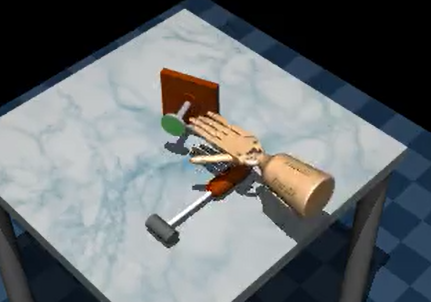
\includegraphics[width=1\linewidth]{C:/MGTU/baseAI/lr12/lr12/bag/report/images/begin.png}
        \caption*{a)}
    \end{minipage}
    \hfill
    \begin{minipage}[H]{0.48\linewidth}
        \centering
        \includegraphics[width=0.99\linewidth]{C:/MGTU/baseAI/lr12/lr12/bag/report/images/took\_hammer.png}
        \caption*{б)}
    \end{minipage}
\end{figure}

\begin{figure}[H]
    \centering
    \begin{minipage}[H]{0.48\linewidth}
      \centering
      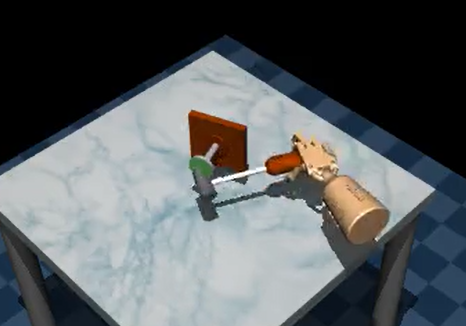
\includegraphics[width=80mm, height=60mm]{C:/MGTU/baseAI/lr12/lr12/bag/report/images/near_gvodz.png}
      \caption*{в)}
    \end{minipage}
    \hfill
    \begin{minipage}[H]{0.48\linewidth}
      \centering
      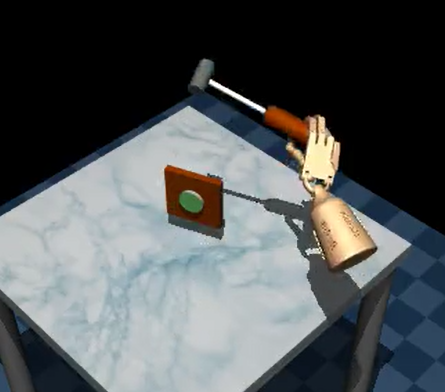
\includegraphics[width=80mm, height=60mm]{C:/MGTU/baseAI/lr12/lr12/bag/report/images/end.png}
      \caption*{г)}
    \end{minipage}
    \caption{Визуализация работы агента: а) начало; б) поднятие молотка; в) молоток возле гвоздя; г) конец}
    \label{fig:work}
  \end{figure}

\section*{Вывод}

В ходе технологической части модель была успешно обучена для решения задачи AdroitHand - Hammer-v1. 
Эта модель может быть использована для управления рукой-роботом, чтобы выполнить задачу забивания гвоздя.
Анализ процесса обучения модели показал, что модель успешно вырабатывает эффективную стратегию для выполнения задачи, 
а тестирование доказало на практике, что агент успешно применяет полученную стратегию для выполнения задачи.

\clearpage
